% Dit werk is gelicenseerd onder de licentie Creative Commons Naamsvermelding-GelijkDelen 4.0 Internationaal. Ga naar http://creativecommons.org/licenses/by-sa/4.0/ om een kopie van de licentie te kunnen lezen.
\documentclass[t]{beamer}

% vaak gebruikte packages, nederlands
\usepackage[margin=2.5cm]{geometry}     % Marges instellen
\usepackage[dutch]{babel}               % Voor nederlandstalige hyphenatie (woordsplitsing)
\usepackage{amsmath,amsthm}             % Uitgebreide wiskundige mogelijkheden
\usepackage{url}                        % Om url's te verwerken
\usepackage{graphicx,subfigure}         % Om figuren te kunnen verwerken
\usepackage{color}
\usepackage{framed}
\usepackage{multicol}
\usepackage[small,bf,hang]{caption}     % Om de captions wat te verbeteren
\usepackage[utf8]{inputenc}             % Om niet ascii karakters rechtstreeks te kunnen typen
\usepackage{float}                      % Om nieuwe float environments aan te maken. Ook optie H!
\usepackage{flafter}                    % Opdat floats niet zouden voorsteken
\usepackage[section]{placeins}			% Om ervoor te zorgen dat floats binnen dezelfde section blijven
\usepackage[nottoc]{tocbibind}			% Bibliografie en inhoudsopgave in ToC; zie tocbibind.dvi
\usepackage{fancyhdr}                   % Voor fancy headers en footers
\usepackage{thmtools}                   % theorem tools
\usepackage{parskip}                    % Om paragrafen met een verticale spatie ipv horizontaal te laten beginnen
\usepackage[plainpages=false]{hyperref} % Om hyperlinks te hebben in het pdfdocument.



%%%%%%%%%%%%%%%%%%%%%%%%%%%%%%
% Algemene instellingen van het document.
%%%%%%%%%%%%%%%%%%%%%%%%%%%%%%
\renewcommand{\baselinestretch}{1.2} 	% De interlinie afstand wat vergroten.
\setcounter{MaxMatrixCols}{50}          % Max 20 kolommen in een matrix


%%%%%%%%%%%%%%%%%%%%%%%%%%%%%%
% Headers en footers
%%%%%%%%%%%%%%%%%%%%%%%%%%%%%%
\pagestyle{fancy}
\fancyhf{}
\renewcommand{\headrulewidth}{0pt}
\fancyhead[RO] {\rightmark}
\fancyhead[LE] {\leftmark}
\fancyfoot[RO,LE] {\thepage}

% no dot after chapter number
\renewcommand{\chaptermark}[1]{
	\markboth{\MakeUppercase{ \chaptername\ \thechapter\quad #1}}{}
}
% no dot after section number
\renewcommand{\sectionmark}[1]{
	\markright{\MakeUppercase{ \thesection\quad #1}}{}
}

% page header and footer style in mainmatter aanpassen
\let\newmainmatter\mainmatter
\renewcommand{\mainmatter}{

	\pagestyle{fancy}
	\fancyhf{}
	\renewcommand{\headrulewidth}{0pt}
	\fancyhead[RO] {\rightmark}
	\fancyhead[LE] {\leftmark}
	\fancyfoot[RO,LE] {\thepage}
	\fancyfoot[C]{\tiny{Brecht Baeten}}

	\newmainmatter
}
\let\newappendix\appendix
\renewcommand{\appendix}{
	\fancyfoot{}
	\fancyfoot[RO,LE] {\thepage}
	\newappendix
}


%%%%%%%%%%%%%%%%%%%%%%%%%%%%%%
% Nieuwe omgevingen
%%%%%%%%%%%%%%%%%%%%%%%%%%%%%%
\definecolor{shadecolor}{gray}{0.95}
\newcounter{voorbeeldcounter}[chapter]
\renewcommand{\thevoorbeeldcounter}{\thechapter.\arabic{voorbeeldcounter}}
\makeatletter
\newenvironment{voorbeeld}
{
\vspace{3mm}
\addtolength{\leftskip}{5mm}
\begin{shaded*}
\vspace{-3mm}
\refstepcounter{voorbeeldcounter}
\noindent
\textbf{Voorbeeld \thevoorbeeldcounter:\\}
%\vspace{-8mm}
%\begin{multicols}{2}
}
{
%\end{multicols}
\end{shaded*}
\addtolength{\leftskip}{-5mm}
}
\makeatother  
    
%%%%%%%%%%%%%%%%%%%%%%%%%%%%%%
% .svg commando's
%%%%%%%%%%%%%%%%%%%%%%%%%%%%%%
% nieuw commando om svg files dynamisch te updaten
%\newcommand{\executeiffilenewer}[3]{%
%\ifnum\pdfstrcmp{\pdffilemoddate{#1}}%
%{\pdffilemoddate{#2}}>0%
%{\immediate\write18{#3}}\fi%
%}
%% nieuw commando om. svg figuren in te voegen
%% Gebruik: \includesvg{path/filename.svg}
%\newcommand{\includesvg}[2][0]{%
%\executeiffilenewer{#2.svg}{#2.pdf}%
%{inkscape -z -C --file=#2.svg %
%--export-pdf=#2.pdf --export-latex}%
%\ifx#10
%	\let\svgwidth\undefined
%\else
%	\def\svgwidth{#1}
%\fi%
%\input{#2.pdf_tex}%
%\ifx \svgwidth\undefined
%\else
%	\let\svgwidth\undefined
%\fi%
%}

% nieuw commando om .fig figuren in te voegen
\newcommand{\includefig}[2][0]{%
\ifx#10
	\let\figwidth\undefined
\else
	\def\figwidth{#1}
\fi%
\input{#2.pdf_tex}%
\ifx \figwidth\undefined
\else
	\let\figwidth\undefined
\fi%
}

%%%%%%%%%%%%%%%%%%%%%%%%%%%%%%
% Packages
%%%%%%%%%%%%%%%%%%%%%%%%%%%%%%

%\usepackage{geometry}              	% 
\usepackage[dutch]{babel}               % Voor nederlandstalige hyphenatie (woordsplitsing)
\uselanguage{dutch}
\languagepath{dutch}
\usepackage{amsmath,amsthm}             % Uitgebreide wiskundige mogelijkheden
\usepackage{url}                        % Om url's te verwerken
\usepackage{graphicx,subfigure}         % Om figuren te kunnen verwerken
\usepackage[utf8]{inputenc}             % Om niet ascii karakters rechtstreeks te kunnen typen
\usepackage[section]{placeins}			% Om ervoor te zorgen dat floats binnen dezelfde section blijven
\usepackage{multicol}
\usepackage[absolute,overlay]{textpos}

%%%%%%%%%%%%%%%%%%%%%%%%%%%%%%
% Layout
%%%%%%%%%%%%%%%%%%%%%%%%%%%%%%
\usetheme{Frankfurt}
\usefonttheme[onlymath]{serif}
\AtBeginSection[]
{
  \begin{frame}
    \frametitle{Inhoud}
    \tableofcontents[currentsection]
  \end{frame}
}

\setbeamertemplate{navigation symbols}{}
\setbeamertemplate{footline}[page number]

%%%%%%%%%%%%%%%%%%%%%%%%%%%%%%
% Title
%%%%%%%%%%%%%%%%%%%%%%%%%%%%%%
\title{Fluïdummechanica}
\author{Brecht Baeten\inst{1}}
\institute{
	\inst{1}%
  		KU Leuven, Technologie campus Diepenbeek,\\ e-mail: brecht.baeten@kuleuven.be
}
\date{\today}
%%%%%%%%%%%%%%%%%%%%%%%%%%%%%%
% Omgevingen
%%%%%%%%%%%%%%%%%%%%%%%%%%%%%%


\subtitle{Inleiding}

\begin{document}
	\frame{\titlepage}
	\begin{frame}
		\frametitle{Inleidende voorbeelden}
		\center
    	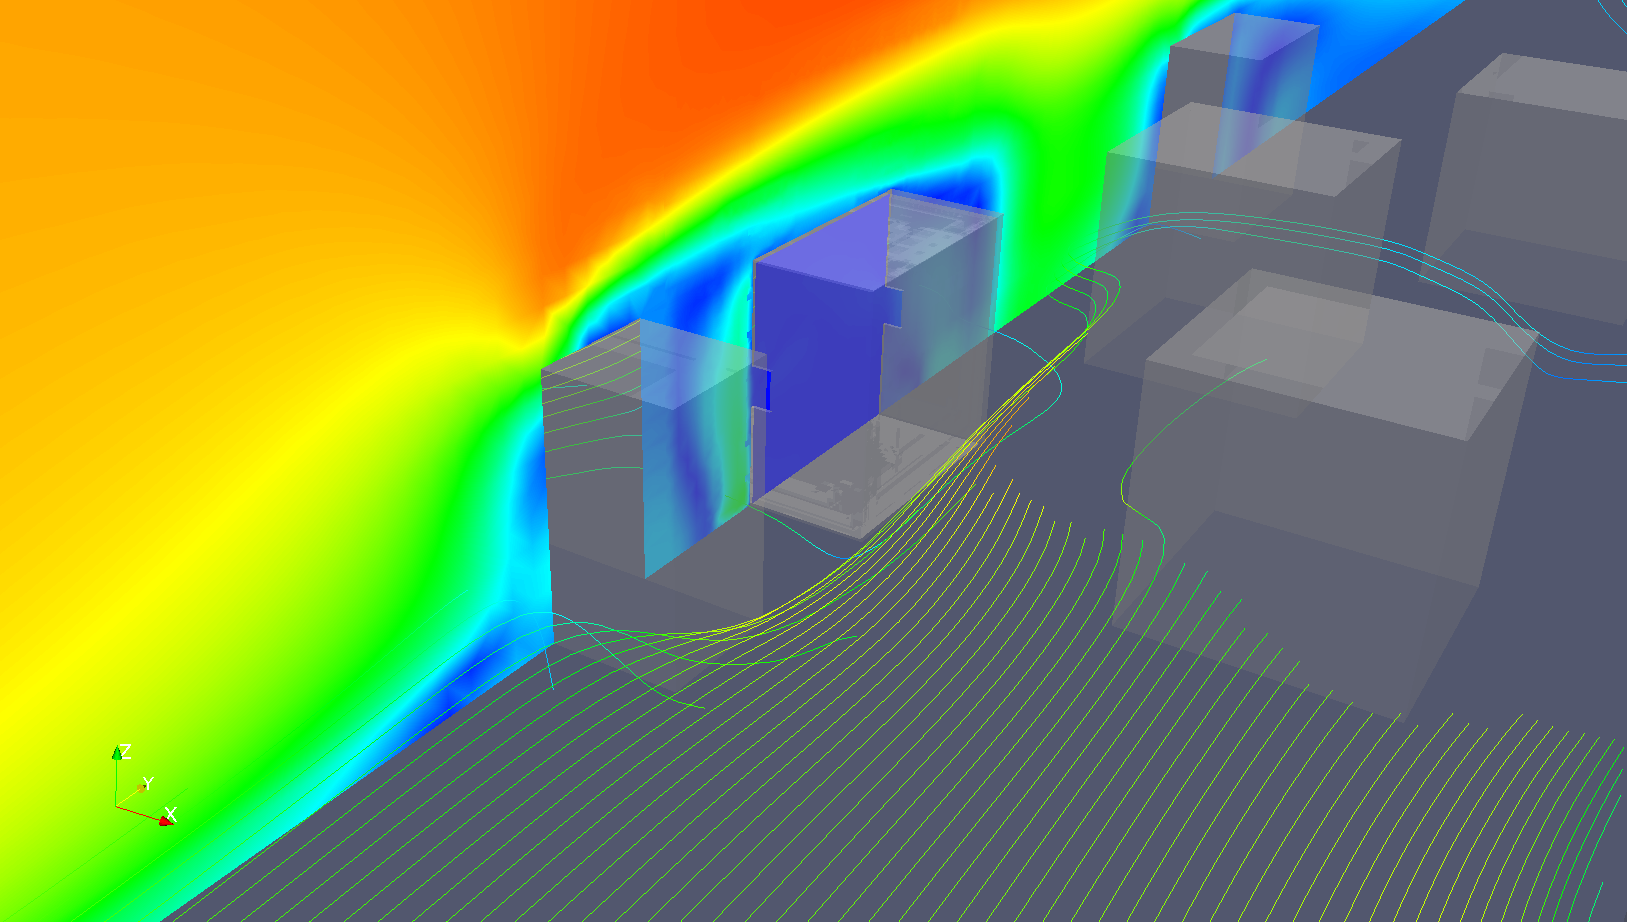
\includegraphics[height=0.7\textheight]{fig/inleiding/building_neighbourhood_cfd}\\
		\footnotesize{Bron: http://www.refresh-project.org.uk/}
  	\end{frame}
%%%%%%%%%%%%%%%%%%%%%%%%%%%%%%%%%%%%%%%%%%%%%%%%%%%%%%%%%%%%%%%%%%%%%%%%%%%%%%%%%
	\begin{frame}
		\frametitle{Inleidende voorbeelden}
		\center
    	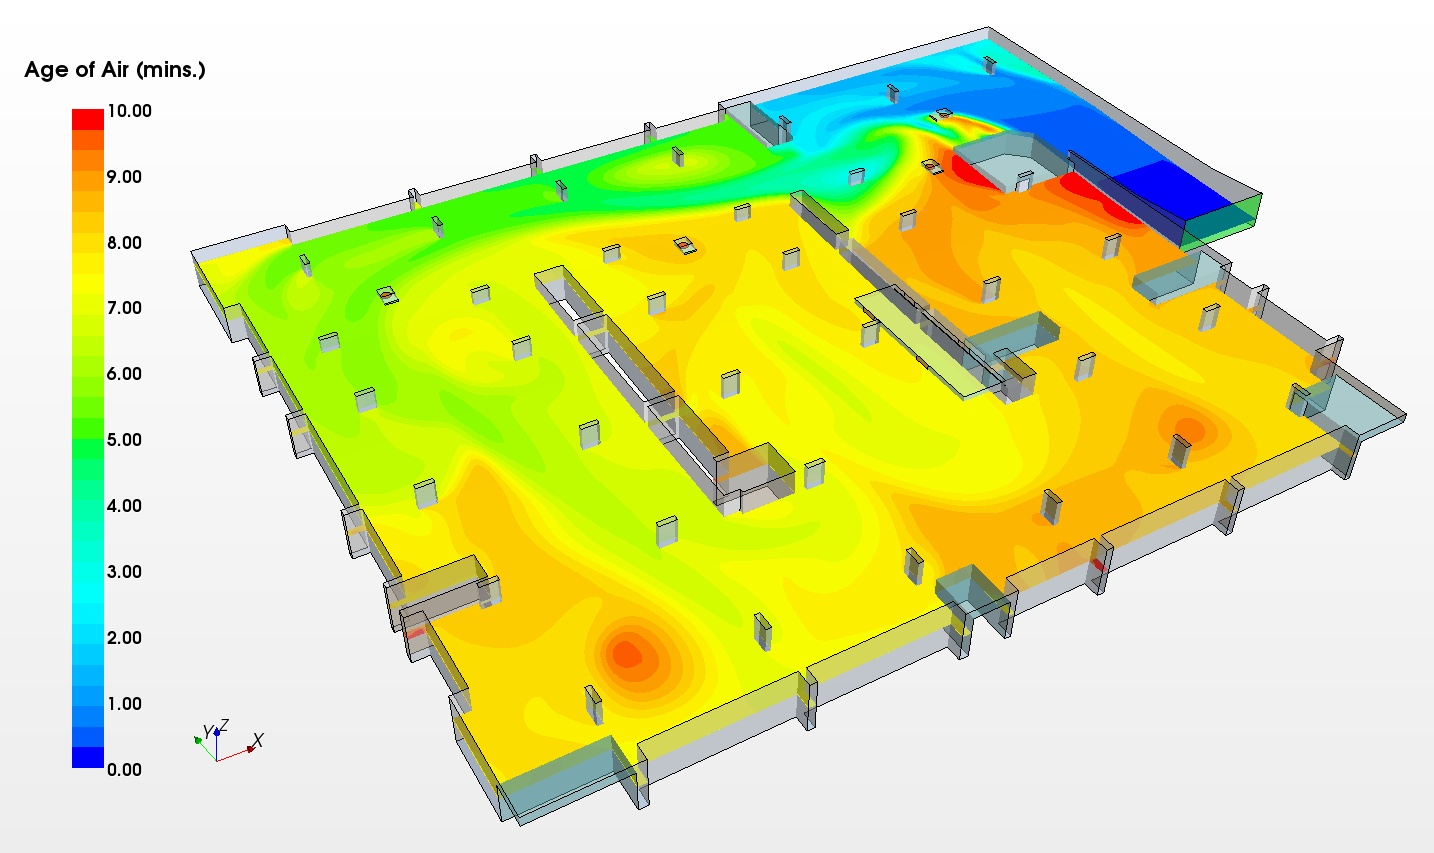
\includegraphics[height=0.7\textheight]{fig/inleiding/ventilation_cfd}\\
		\footnotesize{Bron: https://www.iesve.com/}
  	\end{frame}
%%%%%%%%%%%%%%%%%%%%%%%%%%%%%%%%%%%%%%%%%%%%%%%%%%%%%%%%%%%%%%%%%%%%%%%%%%%%%%%%%
	\begin{frame}
		\frametitle{Inleidende voorbeelden}
		\center
    	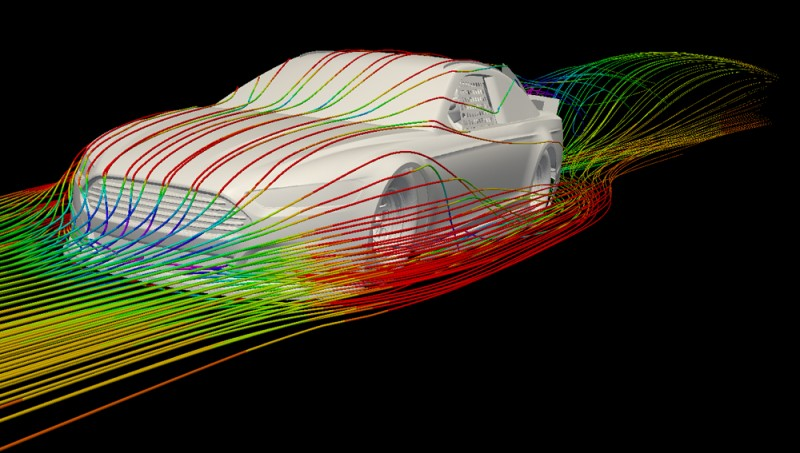
\includegraphics[height=0.7\textheight]{fig/inleiding/Ford-Fusion-CFD}\\
		\footnotesize{Bron: http://en.wikinoticia.com/}
  	\end{frame}
%%%%%%%%%%%%%%%%%%%%%%%%%%%%%%%%%%%%%%%%%%%%%%%%%%%%%%%%%%%%%%%%%%%%%%%%%%%%%%%%%
	\begin{frame}
		\frametitle{Inleidende voorbeelden}
		\center
    	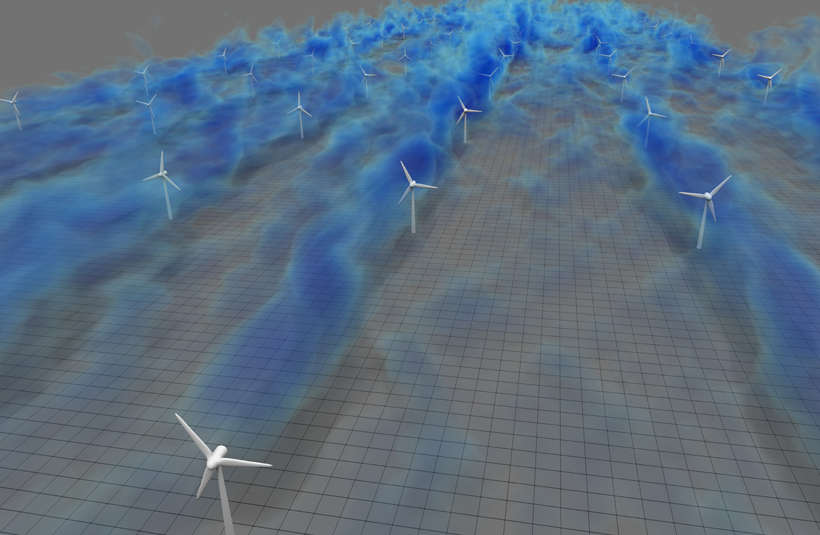
\includegraphics[height=0.7\textheight]{fig/inleiding/JRSE-Stevens-wind_farms}\\
    	\footnotesize{Bron: https://www.aip.org/}
  	\end{frame}
%%%%%%%%%%%%%%%%%%%%%%%%%%%%%%%%%%%%%%%%%%%%%%%%%%%%%%%%%%%%%%%%%%%%%%%%%%%%%%%%%
	\begin{frame}
		\frametitle{Inleidende voorbeelden}
		\center
    	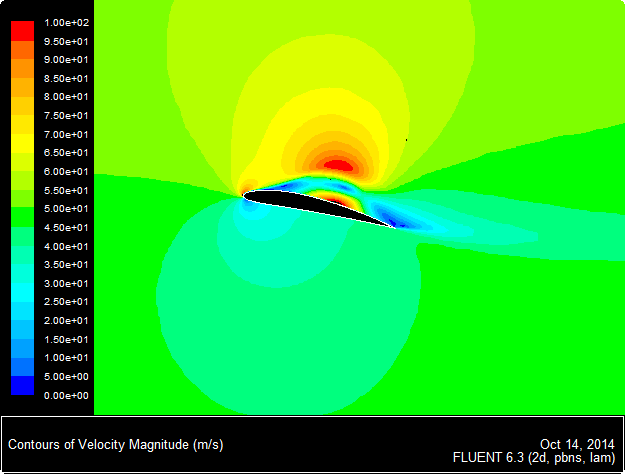
\includegraphics[height=0.7\textheight]{fig/inleiding/NACA4412_velocity_12deg}\\
  	\end{frame}
%%%%%%%%%%%%%%%%%%%%%%%%%%%%%%%%%%%%%%%%%%%%%%%%%%%%%%%%%%%%%%%%%%%%%%%%%%%%%%%%%
	\begin{frame}
		\frametitle{Inleidende voorbeelden}
		\center
    	\includegraphics[height=0.7\textheight]{fig/inleiding/pipingnetwork}\\
    	\footnotesize{Bron: http://blogs.intergraph.com/getsmart/}
  	\end{frame}
%%%%%%%%%%%%%%%%%%%%%%%%%%%%%%%%%%%%%%%%%%%%%%%%%%%%%%%%%%%%%%%%%%%%%%%%%%%%%%%%%
	\begin{frame}
		\frametitle{Project}
		\center
    	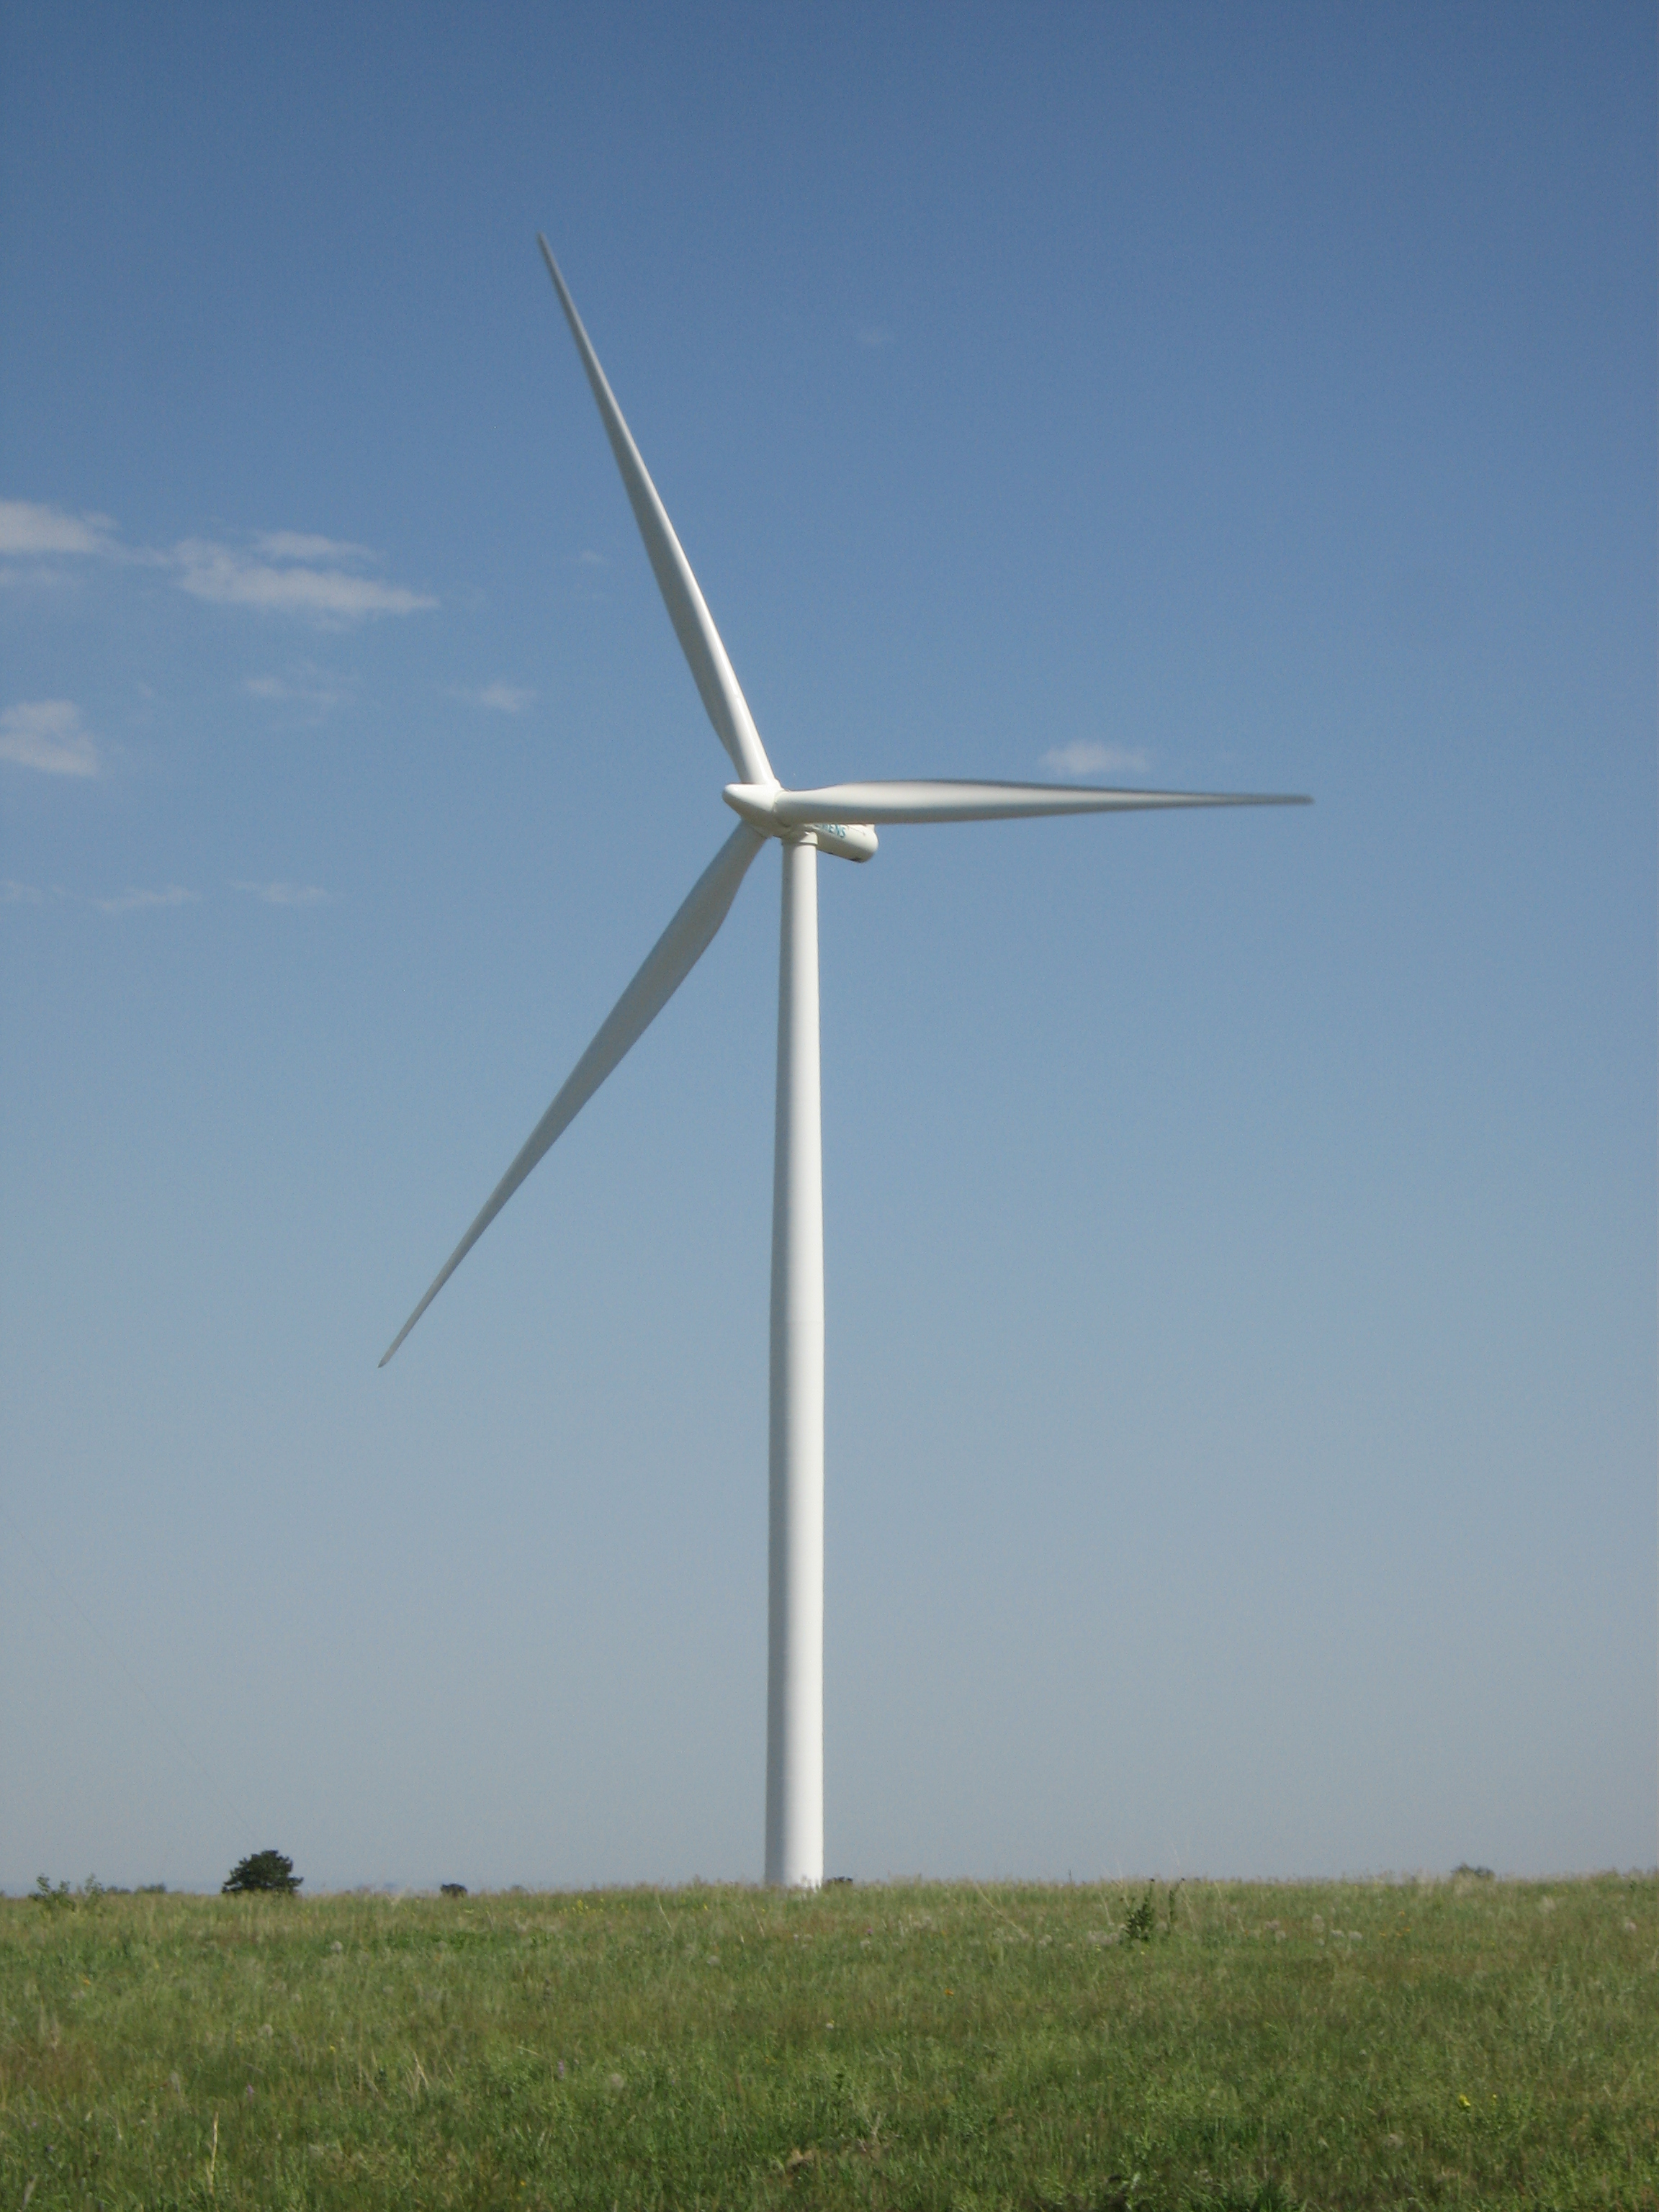
\includegraphics[height=0.8\textheight]{fig/inleiding/wind_turbine_tcm18-88992}\\
    	\footnotesize{Bron: https://www.uml.edu/}
  	\end{frame}  	
%%%%%%%%%%%%%%%%%%%%%%%%%%%%%%%%%%%%%%%%%%%%%%%%%%%%%%%%%%%%%%%%%%%%%%%%%%%%%%%%%
	\begin{frame}
		\frametitle{ECTS Fiche}
		\begin{itemize}
			\item Examen (8/20 toepassingen, 8/20 theorie)
			\item Project (4/20)
		\end{itemize}
		\begin{itemize}
			\item EC1: Kennis van belangrijke begrippen
			\item EC2: Verklaren van stromings fenomenen
			\item EC4: Verzamelen en verwerken van informatie voor het Project
			\item EC5: Analyseren van stromingsproblemen
			\item EC6: Maken van gepaste veronderstellingen en vereenvoudigingen voor de oplossing van stromingsproblemen
			\item EC8: Inschatten van grootteordes bij stromingsproblemen
			\item EC9: Schrijven van een technisch projectverslag
			\item EC12: Gebruik van duidelijke notaties, omgaan met onbekende materie		
		\end{itemize}
  	\end{frame}
%%%%%%%%%%%%%%%%%%%%%%%%%%%%%%%%%%%%%%%%%%%%%%%%%%%%%%%%%%%%%%%%%%%%%%%%%%%%%%%%%
\end{document}